This section describes the chosen research method for this study. As discussed in the previous section, the chosen method was case study. Yin defines, in \cite{CaseStudyResearch}, a case study in the following way:

\begin{enumerate}
\item A case study is an empirical inquiry that
\begin{itemize}
\item investigates a contemporary phenomenon in depth and within its real-life context, especially when
\item the boundaries between a phenomenon and context are not clearly evident.
\end{itemize}
\item The case study inquiry
\begin{itemize}
\item copes with the technically distinctive situation in which there will be many more variables of interest than data points, and as one result
\item relies on multiple sources of evidence, with data needing to converge in a triangulating fashion, and as another result
\item benefits from the prior development of theoretical propositions to guide data collection and analysis.
\end{itemize}
\end{enumerate}

The research process is illustrated in figure \ref{fig:caseProcess}. As the figure shows, the process in linear, but iterative. This means that one can go back to previous phases if one sees the need for that. The Plan phase consisted of  identifying research questions and deciding to use case study as the research method for this study. The design phase is about getting from initial questions to conclusions or answers. It is the logic that links the data to be collected to the initial questions of the study \cite{CaseStudyResearch}. 

\begin{figure}[H]
\begin{center}
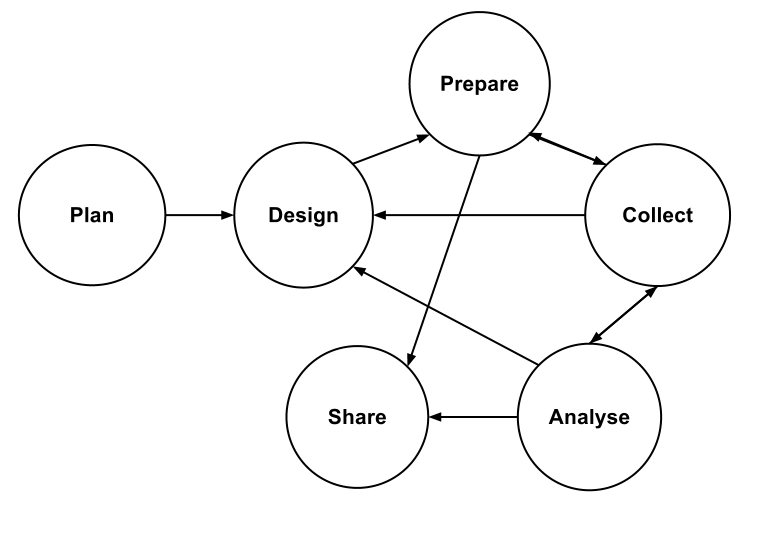
\includegraphics[scale=0.38]{caseProcess.png}
\caption[Case Study Research Process]{The linear, but iterative process of doing case study research \cite{CaseStudyResearch}}
\label{fig:caseProcess}
\end{center}
\end{figure}

The case design has five important components \cite{CaseStudyResearch}:

\begin{enumerate}
\item A study's questions
\item Its propositions, if any
\item Its unit(s) of analysis
\begin{enumerate}
\item What is the case?
\end{enumerate}
\item The logic linking the data to the propositions
\begin{enumerate}
\item analytic techniques, should be known prior to the data collection, so the right data will be collected
\end{enumerate}
\item The  criteria for interpreting the findings
\begin{enumerate}
\item The challenge is to anticipate and enumerate the important rival explanations for the findings
\end{enumerate}
\end{enumerate}

Yin presents, in \cite{CaseStudyResearch}, four tactics to maximize the quality of empirical research. These tactics are applied to four different tests as shown in figure \ref{fig:caseTactics}. The test for internal validity is not so relevant for this study, as it is mainly an \textit{exploratory} study.
%Bør vel endre på denne evt fjerne, vi gidder jo ikke følge alle disse tacticsene + at nr 2 kanskje ikke er så relevant for oss

\begin{figure}[H]
\begin{center}
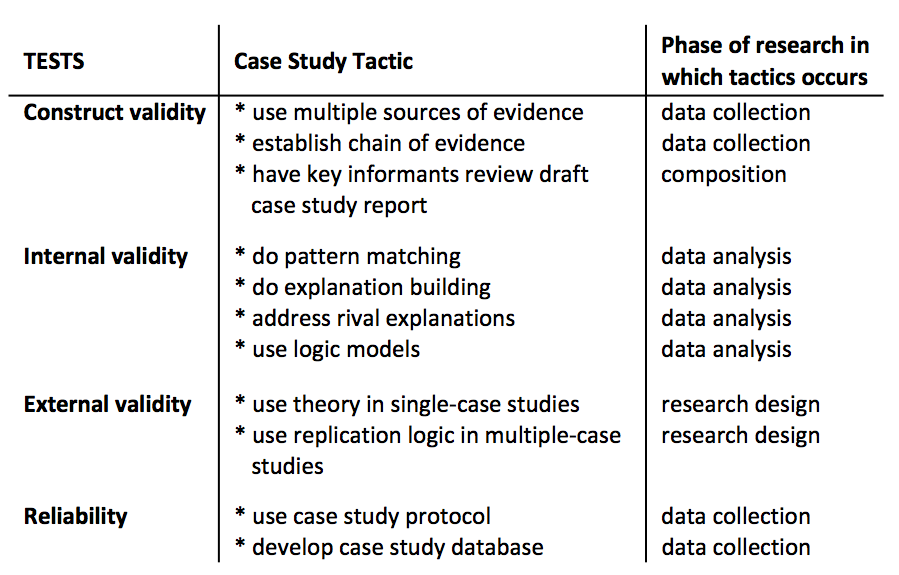
\includegraphics[scale=0.82]{caseTactics.png}
\caption[Case Study Tactics for Four Design Tests]{Case Study Tactics for Four Design Tests \cite{CaseStudyResearch}}
\label{fig:caseTactics}
\end{center}
\end{figure}

The choice between a single- and multiple-case also belongs to the design phase. Multiple-case is usually preferred \cite{CaseStudyResearch} and it was chosen as the method for this study. Additionally each case may be embedded or holistic. An embedded case has more than one unit of analysis. The design for this study is a mix, a multiple-case with both an embedded and a holistic case. %NB, dette kan endres!!!! Multiple: select each case so that it either (a) predicts similar results (literal replication) or (b) predicts contrasting results but for anticipatable reasons (theoretical replication). Dette har vel ikke vi gjort
The design is illustrated in figure \ref{fig:caseDesign}.

\begin{figure}[H]
\begin{center}
\includegraphics[scale=0.685]{caseStructure.png}
\caption[Case Design for this Study]{Case Design for this Study, modified from \cite{CaseStudyResearch}}
\label{fig:caseDesign}
\end{center}
\end{figure}

The preparation phase was very important for us as we do not have experience with the case study research method. The main activities performed in this phase were related to acquiring the desired skills and to prepare for the specific case studies. It is considered difficult to acquire desired skills of being a case study investigator because procedures are not routinised. It is advised to prepare to ask good questions, be a good "listener", be adaptive and flexible, have a firm grasp of the issues being studied and be unbiased by preconceived notions. We have performed a background study in order to get a thorough understanding of the issues in the study.